% ------------------------------------------------------------------------------
% TYPO3 Version 10.4 - What's New (German Version)
%
% @license	Creative Commons BY-NC-SA 3.0
% @link		https://typo3.org/help/documentation/whats-new/
% @language	German
% ------------------------------------------------------------------------------

\section{Änderungen für Integratoren}
\begin{frame}[fragile]
	\frametitle{Änderungen für Integratoren}

	\begin{center}\huge{Kapitel 2:}\end{center}
	\begin{center}\huge{\color{typo3darkgrey}\textbf{Änderungen für Integratoren}}\end{center}

\end{frame}

% ------------------------------------------------------------------------------
% Feature | 89513 | Provide password recovery for backend users

\begin{frame}[fragile]
	\frametitle{Änderungen für Integratoren}
	\framesubtitle{E-Mail zur Passwort-Wiederherstellung (1)}

	\begin{itemize}

		\item Passwortrücksetzungen für Backend-Benutzer sind nur 4 Stunden lang gültig. Dieses Zeitlimit ist nicht konfigurierbar.
		\item Um die Sicherheit zu erhöhen, kann die Funktion für Admin-Benutzer oder für alle Benutzer deaktiviert werden.
		\item Wenn Benutzer eine E-Mail-Adresse gemeinsam nutzen, wird ein alternativer E-Mail-Text verwendet.
		\item Das TCA-Feld \texttt{be\_users.email} darf nicht auf \texttt{eval=email} gesetzt werden.

		\item Die Funktion wirkt nur für Benutzer, die:
			\begin{itemize}
				\item eine E-Mail-Adresse eingestellt haben,
				\item ein Passwort gesetzt haben, und
				\item sind nicht deaktiviert/gelöscht.
			\end{itemize}

	\end{itemize}

\end{frame}

% ------------------------------------------------------------------------------
% Feature | 89513 | Provide password recovery for backend users

\begin{frame}[fragile]
	\frametitle{Änderungen für Integratoren}
	\framesubtitle{E-Mail zur Passwort-Wiederherstellung (2)}

	\begin{itemize}
		\item Passwort-Wiederherstellungs-E-Mails können auch auf der Befehlslinie ausgelöst werden.
	\end{itemize}

	\begin{figure}
		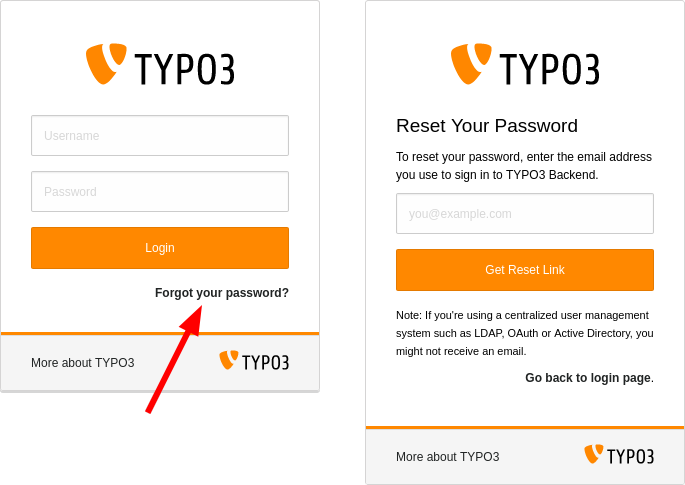
\includegraphics[width=0.9\linewidth]{ChangesForIntegrators/89513-ProvidePasswordRecoveryForBackendUsers.png}
	\end{figure}

\end{frame}

% ------------------------------------------------------------------------------
% Important | 90285 | Fresh installs without constraint for typo3fluid/fluid will get version 3.0+

\begin{frame}[fragile]
	\frametitle{Änderungen für Integratoren}
	\framesubtitle{Fluid-Templating-Engine}

	\begin{itemize}
		\item Der TYPO3-Kern ist vollständig kompatibel mit Fluid Version 2.6+ und 3.0+
		\item Bei Neuinstallationen ohne Abhängigkeitssatz wird Fluid Version 3.x
			(\texttt{typo3fluid/fluid:\^{}3}) heruntergeladen und installiert.
		\item Wenn Ihr Projekt Fluid-Vorlagen enthält, die mit Version 3.0+ inkompatibel sind,
			ergreifen Sie eine der folgenden Maßnahmen:

			\begin{itemize}
				\item Begrenzen Sie die maximale Version: \texttt{typo3fluid/fluid:\^{}2}
				\item Aktualisieren Sie Ihre Fluid-Vorlagen.
			\end{itemize}

	\end{itemize}

\end{frame}

% ------------------------------------------------------------------------------
% Important | 18079 | pages.doktype restriction for frontend queries refined

\begin{frame}[fragile]
	\frametitle{Änderungen für Integratoren}
	\framesubtitle{Behandlung von Seitentypen}

	\begin{itemize}
		\item Die interne Behandlung von Seitentypen in TYPO3 hat sich geändert.
		\item Die Option \texttt{pages.doktype} bezeichnet einen numerischen Wert, der den Typ,
			z.B. Standardseite, Ordner, Verknüpfung, Link zu externer URL, usw.
		\item Seiten bestimmter Typen (z.B. Ordner und Recycler) wurden ausgeschlossen, wenn Inhalte
			von einer bestimmten Seite gelesen oder Datensätze abgerufen wurden.
		\item Diese Einschränkung wurde nun aufgehoben, und benutzerdefinierte Seiten-Doktypen mit einer 
			Nummer >200 sind nun möglich.
		\item Integratoren und Entwickler, die Seiten-Doktypen verwendet haben, z.B. in TypoScript,
			wird empfohlen, zu überprüfen, ob das frühere Verhalten missbraucht wurde und jetzt eine Aktualisierung erfordert.
	\end{itemize}

\end{frame}

% ------------------------------------------------------------------------------
% Feature | 90826 | Compare backend usergroups

\begin{frame}[fragile]
	\frametitle{Änderungen für Integratoren}
	\framesubtitle{Backend-Benutzer-Modul}

	\begin{itemize}
		\item Integratoren sind jetzt in der Lage, einzelne Backend-Benutzergruppen zu vergleichen.
	\end{itemize}

	\begin{figure}
		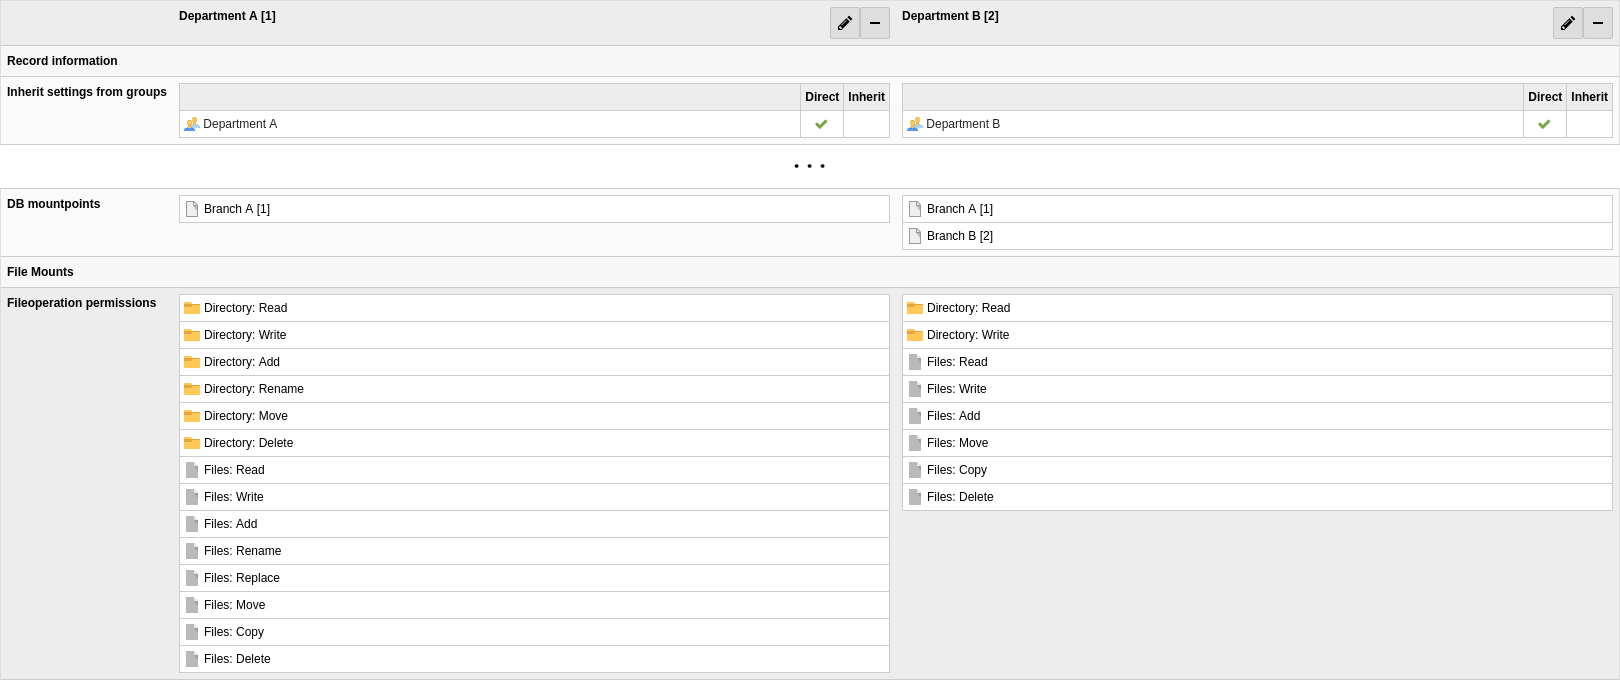
\includegraphics[width=0.9\linewidth]{ChangesForIntegrators/90826-CompareBackendUsergroups.png}
	\end{figure}

\end{frame}

% ------------------------------------------------------------------------------
% Important | 89555 | Workspace-related database records contain the proper Page ID

\begin{frame}[fragile]
	\frametitle{Änderungen für Integratoren}
	\framesubtitle{Workspaces}

	\begin{itemize}
		\item Viele Jahre lang setzte der TYPO3-Kern \texttt{pid} auf \texttt{-1} der unveröffentlichten Datensätze.
		\item TYPO3 verarbeitet nun versionierte Datensätze durch Validierung der folgenden drei Felder:

			\begin{itemize}
				\item \texttt{t3ver\_wsid} (the workspace ID the record is versioned in)
				\item \texttt{t3ver\_state} (the type of the versioned record)
				\item \texttt{t3ver\_oid} (the live version of a record)
			\end{itemize}

		\item Daher ist \texttt{pid=-1} nicht mehr erforderlich.
		\item Der Upgrade-Wizard konvertiert alle \texttt{pid}-Felder von versionierten Datensäten
			in realen \texttt{pid}-Werte.
		\item Neue Anlagen sind von dieser Änderung nicht betroffen.

	\end{itemize}

\end{frame}

% ------------------------------------------------------------------------------
% Deprecation | 91030 | Runtime-Activated Packages

\begin{frame}[fragile]
	\frametitle{Änderungen für Integratoren}
	\framesubtitle{Laufzeit-aktivierte Pakete}

	\begin{itemize}
		\item Die folgende globale Konfigurationsoption wurde als \textbf{veraltet} markiert:\newline
			\smaller
				\texttt{\$GLOBALS['TYPO3\_CONF\_VARS']['EXT']['runtimeActivatedPackages']}
			\normalsize
		\item Die Verwendung von laufzeitaktivierten Erweiterungen verlangsamt eine TYPO3-Instanz erheblich.
		\item Integratoren wird empfohlen, die notwendigen Schritte einzuleiten, wenn solche Warnungen
			im Verwerfungsprotokoll erscheinen:\newline
			\begingroup
				\fontsize{8}{10}
				\texttt{Die Unterstützung für Laufzeit-aktivierte Pakete wird in TYPO3 v11.0 entfernt.}
			\endgroup

	\end{itemize}

\end{frame}

% ------------------------------------------------------------------------------
